% meta.concepts: truss
% meta.tags: realistic
% acknowledge: Peter Seiler & Luke Melander graciously shared Spring 2019 course material
% source: 2019 P. Seiler AEM2011 HW 9

The rear landing gear mechanism from the Airbus A400M military transport aircraft is shown below. The
simplified diagram provided shows the external forces acting on the mechanism during the final phase of a
landing. Each of the three sections of the mechanism have identical dimensions. The mechanism is connected
to the aircraft with a fixed support at point A and a roller support at point B. Determine the internal forces
at point D, which is the midpoint of member AC.

\begin{figure}[ht!]
  \centering
  \includegraphics[width=0.4\textwidth,
	           height=0.3\textheight,
		   keepaspectratio]{figa.png}
  \includegraphics[width=0.4\textwidth,
	           height=0.3\textheight,
		   keepaspectratio]{figb.png}
  \caption*{A400M Rear Landing Gear (left) Simplified Diagram (right)}
\end{figure}

\iftoggle{flagSoln}{%
\vspace{.5cm}
\rule{\textwidth}{.4pt}
\vspace{.5cm}
\textbf{Solution:}
\begin{figure}[ht!]
  \centering
  \frame{\includegraphics[width=0.9\textwidth,
	           height=0.3\textheight,
       keepaspectratio]{solna.png}}
  \frame{\includegraphics[width=0.9\textwidth,
	           height=0.3\textheight,
       keepaspectratio]{solnb.png}}
  \frame{\includegraphics[width=0.9\textwidth,
	           height=0.3\textheight,
       keepaspectratio]{solnc.png}}
\end{figure}
}{%
}%
